% !TEX root = main.tex

\documentclass{Interspeech}

\usepackage{todonotes}
\usepackage{hyperref}
\usepackage{mathrsfs}
\hypersetup{
    colorlinks=true,
    linkcolor=black,
    filecolor=magenta,      
    urlcolor=red,
    pdftitle={Defence Against the Deepfake Arts},
    pdfpagemode=FullScreen,
    references=true,  
}

% 2023-10-21 modified by Simon King (Simon.King@ed.ac.uk)  
% 2024-01 modified by TPC Chairs of Interspeech 2024  
% 2024-10 modified by Antoine Serrurier for Interspeech 2025
% 2024-12 modified by TPC Chairs of Interspeech 2025
% 2025-02 modified by Team DADA

% ************************************* *
% *    DOUBLE-BLIND REVIEW SETTINGS    *
% **************************************
% Comment out \interspeechcameraready when submitting the 
% paper for review.
% If your paper is accepted, uncomment this to produce the
%  'camera ready' version to submit for publication.

% \interspeechcameraready


% **************************************
% *                                    *
% *      STOP !   DO NOT DELETE !      *
% *          READ THIS FIRST           *
% *                                    *
% * This template also includes        *
% * important INSTRUCTIONS that you    *
% * must follow when preparing your    *
% * paper. Read it BEFORE replacing    *
% * the content with your own work.    *
% **************************************

% title here must exactly match the title entered into the paper submission system
\title{Defence Against the Deepfake Arts : Improving Audio Deepfake Detection With Context Awareness}

% the order of authors here must exactly match the order entered into the paper submission system
% note that the COMPLETE list of authors MUST be entered into the paper submission system at the outset, including when submitting your manuscript for double-blind review
\author[affiliation={1, 2*}]{Nicoline}{Nymand-Andersen}
\author[affiliation={1*}]{Ivanina}{Ivanova}
\author[affiliation={1*}]{Abhay}{Dayal Mathur}
\author[affiliation={1}]{Nils}{Holzenberger}


%The maximum number of authors in the author list is 20. If the number of contributing authors is more than this, they should be listed in a footnote or the acknowledgement section.

% if you have too many addresses to fit within the available space, try removing the "\\" newlines
\affiliation{Telecom Paris}{Institut Polytechnique de Paris}{France}
\affiliation{Department of Computer Science}{Technische Universität München}{Germany}
% \affiliation{}{Just Institute}{And Country}
\email{nnymand-23@ip-paris.fr, ivanina.ivanova@ip-paris.fr, abhay.mathur@ip-paris.fr, nils.holzenberger@telecom-paris.fr}
\keywords{audio deepfake detection}

\newcommand{\blue}[1]{\textcolor{blue}{#1}}
\usepackage{comment}

\begin{document}

\maketitle

% the abstract here must exactly match the abstract entered into the paper submission system
\begin{abstract}

  % 1000 characters. ASCII characters only. No citations.
  \todo[inline]{Abhay : 1000 character limit; 848 currently.}
  The increasing use of generative AI models to create realistic deepfakes poses significant challenges to information security, particularly in the realm of audio manipulation. This paper addresses the pressing need for improved detection of audio deepfakes by proposing a novel approach, DADA, that leverages textual context extracted from transcriptions as well as audio features extracted from deepfake detection models. We propose two fusion strategies, late fusion and mid fusion, to integrate these features and enhance detection accuracy. We conduct experiments using benchmark datasets and state-of-the-art deepfake detection models to evaluate the performance of our proposed approach. Our results demonstrate promising improvements in detecting audio deepfakes, highlighting the potential of context awareness in enhancing detection capabilities.
\end{abstract}

\section{Introduction}
\label{sec:introduction}

With the rapid advances in the digital landscape and new media technologies,
users become increasingly exposed to different types of manipulations.
Nowadays, everyone can create highly realistic AI-generated content such as
images, audio, and even videos. Distinguishing between those and the real ones
becomes nearly impossible for the ordinary user. Audio deepfakes or voice
clones are like digital ventriloquists, using various deep learning techniques
to create voices that convincingly impersonate real people~\cite{adversarial}.
We can distinguish between a couple of different types of deepfakes.
~\cite{review_audio_deepfake_issues}. The first approach is imitation-based
(voice conversion), wherein the original audio signal is modified to mimic
another targeted voice. This technique is mainly used in show business and,
therefore, is applied by a third person or deep learning software. The next
approach is synthetic-based, producing artificially generated speech using
text-to-speech techniques (TTS). This process involves three stages: text
analysis, acoustic, and vocoder. The third technique is centred on replaying
existing recordings of the target speaker. Two techniques are notable here:
cut-and-paste detection, where a victim's recorded segment is played through a
phone handset for capture, and far-field detection, which involves crafting
sentences for manipulation of a text-dependent system. There are other types of
deepfakes, such as emotion fake. This technique alters the emotions of a
speaker's voice while preserving the original words and speaker identity.
~\cite{zhao2023emofake}. Another type is scene fake, which involve modifying
the background sounds of a recording, leaving the speaker and content
untouched.~\cite{yi2022scenefake}. The last type of deepfake is the partially
fake, which involves replacing specific words within the original audio signal
with either real or synthetic audio segments. The speaker remains the same
throughout, but the content is altered~\cite{yi2023halftruth}.

\begin{figure}[t]
  \centering
  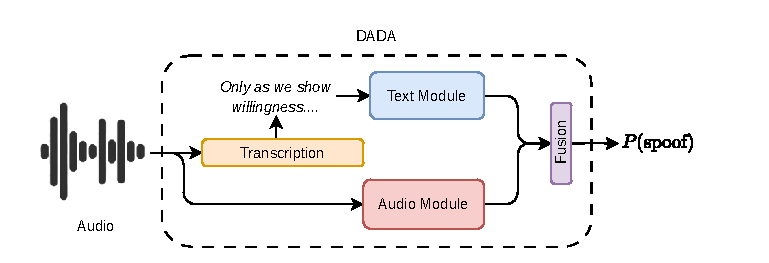
\includegraphics[width=0.5\textwidth]{figures/overview.pdf}
  \caption{Overview of the DADA pipeline. Audio files are first transcribed to obtain textual content. Features are then extracted from both the audio and text using separate models. Finally, these features are combined (using either mid fusion or late fusion strategies) to generate the final prediction.}\label{fig:overview}
\end{figure}

All these different techniques can have far-reaching consequences, affecting
domains ranging from political discourse to personal security. These deepfakes
are not only used in creating political propaganda to manipulate public
opinion~\cite{stuanescuinformational} but have also become tools for conducting
phone scams~\cite{mirsky2022dfcaptcha}, posing significant threats to
individual privacy and security. The ability to convincingly replicate or alter
voices using AI have affirmed the urgent need for robust detection mechanisms.
This paper contributes to proactive measures in detecting audio deepfakes,
particularly focusing on detecting audio deepfakes of public figures. Public
figures are especially susceptible to the detrimental effects of audio
deepfakes as their extensive online presence renders them prime targets for
malicious actors seeking to disseminate misinformation.

We propose a new pipeline that aims to not only analyze the audio utterances
but also incorporate contextual information. Furthermore, DADA has two
different branches, one responsible for detecting if the audio is real or fake
and a text branch performing the task of Authorship Attribution on the
transcription of the audio. We want to answer the question of what is the
probability of the anticipated speaker having made the given statement.
% changelog[Abhay]: removed the abbreviation AA here, as it is not used in the text later + Alcoholics Anonymous prolly has dibs

Recent advancements in authorship attribution using deep learning have
showcased the efficacy of various encoder-based architectures in capturing
linguistic and stylistic patterns unique to individual authors. We can
encounter multiple papers that explore BERT or T5-based models for identifying
authorship in literary texts, achieving notable
accuracy~\cite{hicke2023t5,silva2024forged}. For instance,
BertAA~\cite{fabien2020bertaa} is a fine-tuned pretrained BERT model for
authorship attribution, demonstrating competitive performance on multiple
datasets. We can also find several papers that use techniques from contrastive
learning in creating discriminative embedding spaces. Works like
DeepStyle ~\cite{hu2020deepstyle}, focusing on short-text authorship
attribution, leveraging Triplet Loss, which outperformed existing baselines
using Twitter and Weibo datasets and using Siamese networks for large-scale
author identification~\cite{saedi2021siamese}. A transformer-based model ~\cite{bauersfeld2023cracking} are used also for authorship attribution on arXiv manuscripts, achieving high attribution accuracy in a large-scale dataset with up to 2,000 authors.

\section{Related Work}\label{sec:related_work}
\todo[inline]{Keeping all related work in Introduction~\ref{sec:introduction} for now, in line with papers from Interspeech24.}

\section{Method}\label{sec:method}

In this section, we present the DADA architecture for audio deepfake detection
that improves the traditional methods analyzing only the utterances of the
audio files, by incorporating contextual information to improve detection
capabilities. Specifically, our approach seeks to determine not only whether an
audio sample is a deepfake but also the likelihood of the supposed speaker
having made the given statement, thus embedding contextual awareness into the
detection pipeline. An overview of the pipeline is shown in
Figure~\ref{fig:overview}.

Our method operates in three stages: transcription, feature extraction and
fusion. First, the audio files are transcribed using
Whisper~\cite{radford2023robust} to obtain the textual content. Following
transcription, the architecture leverages two separate models trained
independently a text and an audio model. The extracted audio and text feature
are then combined using two distinct fusion strategies to obtain the final
classification score.
% \subsection{Audio Model}
\subsection{Text Model}

The main idea of the text model is to fine-tune a pretrained encoder-based LLM
for authorship attribution. To improve the model's ability to differentiate
between stylistic and linguistic patterns unique to specific author, we
extracted the features from the last three hidden states of the encoder,
instead of only the CLS token. Transformer models encode information
hierarchically across layers. The lower layers capture phrase-level or
segment-level interactions, where the intermediate layers represent syntactic
information like grammar and vocabulary and the higher layers encode
task-specific or abstract semantic information. By using multiple layers we
want capture a broader spectrum of features, combining syntactic, semantic, and
task-specific information~\cite{jawahar2019does}. The extracted features are
aggregated using a Mean Pooling layer, which computes the mean while accounting
for the attention mask. This vector is passed to task-specific layers, such as
a several fully connected layers. To model the space of authors effectively and
identify the characteristics of their speech sets, we employ techniques from
contrastive learning such as Triplet loss. This loss function helps create a
well-defined embedding space, where texts attributed to the same author are
closer together, while those from different authors are further
apart~\cite{mao2019metric}. The function is defined using triplets (A,P,N),
where A is a randomly sampled anchor (reference point), P is a positive sample
that has the same label as A and N is the negative sample of a different random
class than the anchor. The goal is to ensure that the distance between the
anchor and the positive is smaller than the distance between the anchor and the
negative by at least a certain margin $\lambda$. We define the function as follows:

\todo[inline]{Abhay: Aliter}
We define the loss on features $f_\theta^{A}$, $f_\theta^{P}$ and $f_\theta^{N}$ generated by the model on a triplet as follows:

\todo[inline]{changelog[Abhay]: added label, modified notation to reduce width}
\begin{align}
  \mathcal{L} = [d(f_\theta^{A},f_\theta^{P}) - d(f_\theta^{A},f_\theta^{N}) + \lambda]_{+}
  \label{eq:triplet_loss}
\end{align}

% $$\mathscr{L} = \sum_{i=1}^N max[d(f(A^i), f(P^i))- d(f(A^i), f(N^i))+ \lambda, 0]$$

Where $f_\theta(x)$ is the embedding of the input x generated by the model,
$\lambda$ is the margin that enforces a minimum separation between similar and
dissimilar pairs, $d(x,y)$ is the distance function between the two embeddings,
and $[\cdot]_{+} = \max(\cdot, 0)$. We experimented with two different distance
functions, the squared Euclidean distance (L2-norm) and the cosine similarity
between the features.

\subsection{Audio Model}

% Architecture
The audio model uses a Wav2Vec2~\cite{wav2vec2} backbone for feature
extraction, which allows learning representations directly from raw audio
waveforms. To capture a comprehensive set of features, multiple layers from the
model are pooled into a single feature vector. This pooling is achieved using a
compression module that employs attentive mean pooling, which allows the model
to focus on the most informative parts of the audio signal. Additionally,
following~\cite{slim}, a non-linear bottleneck is applied to further refine the
feature vector, ensuring that it captures the essential characteristics needed
for accurate deepfake detection. \todo[inline]{Abhay: not sure if using
  citations independently is consistent/recommended.}
% 

% Training

Similar to the text module, audio features (denoted as $f_{\phi}$) are trained using Contrastive
Learning, with a triplet loss as in Equation~\ref{eq:triplet_loss} using the
cosine distance function. To optimize the margin used in the triplet loss
function, we employ an iterative process that involves three stages: initial
training with a fixed margin, adaptive margin adjustment, and final training
with a fixed margin.

% \subsubsection{Initial Training with Fixed Margin}
In the first stage, we train the model for a few epochs using an a priori fixed
margin, $\lambda_0$. This initial training helps achieve some separation
between classes and provides a good starting point for further optimization.

% \subsubsection{Adaptive Margin Adjustment}
Next, we train the model for additional epochs using an adaptive triplet loss
introduced in~\cite{adatriplet}. \todo[inline]{Abhay: Again, using citation
  independently.} This
constitutes adding an additional soft constraint on the virtual angle between
the anchor and the negative sample using another margin $\lambda'$ as follows.

\begin{align}
  \begin{split}
    \mathcal{L}_{ada} & = [d(f_\phi^{A},f_\phi^{P}) - d(f_\phi^{A},f_\phi^{N})+ \lambda]_{+} \\
                      & + [d(f_\phi^{A},f_\phi^{N}) + \lambda']_{+}
  \end{split}
\end{align}

% \subsubsection{Final Training with Fixed Margin}
In the final stage, we fix the margin as the final margin obtained from the
adaptive stage, $\lambda_{f}$, and train the model for a couple more epochs to
achieve optimal performance.

\subsection{Fusion Strategies}
After independently training the audio and text models, we freeze their
parameters and combine their features using one of two fusion strategies: mid
fusion or late fusion.

\subsubsection{Mid Fusion}
In this strategy, the extracted features from the audio and text models are
concatenated to create a joint representation. This combined representation is
then passed through a Multi-Layer Perceptron (MLP) network. The MLP learns to
integrate the audio and text features effectively to make a final prediction.
The training of the MLP is guided by the Binary Cross-Entropy (BCE) loss
function, which is appropriate for binary classification tasks such as
distinguishing between real and spoof audio samples. With this approach we hope
that one of the branches will compensate for the mistakes of the other and
hopefully increase the performance of the detector.

\subsubsection{Late Fusion}
In this approach, the audio and text models are treated as independent
branches, and each produces its own prediction score. The final prediction is
obtained by taking the weighted mean of the scores from the two branches. This
simple averaging method ensures that the final decision benefits from the
independent contributions of both modalities while maintaining the
interpretability of individual scores.

\todo[inline]{!!! Abhay: Need to discuss this}

We model late fusion for two possible scenarios: one where there exists a
purported speaker (consistent with deepfakes claiming to be a specific
individual/celebrity) and one where the speaker is unknown. In the former case,
the text model outputs the probability of the anticipated speaker having made
the given statement, while the audio model predicts the likelihood of the audio
being real or fake. In the latter case, the text model predicts the probability
of the speaker being any of the known authors, while the audio model predicts
the likelihood of the audio being real or fake. The final prediction is
obtained by taking the weighted mean of the scores from the two branches. This
simple averaging method ensures that the final decision benefits from the
independent contributions of both modalities while maintaining the
interpretability of individual scores.

Formally, \todo[inline]{Abhay: I'll complete this today [21.01].}

Both fusion strategies provide distinct advantages: mid fusion enables the
model to learn deeper interactions between the modalities, while late fusion
offers simplicity and preserves the autonomy of each model.

\begin{figure*}[t]
  \centering
  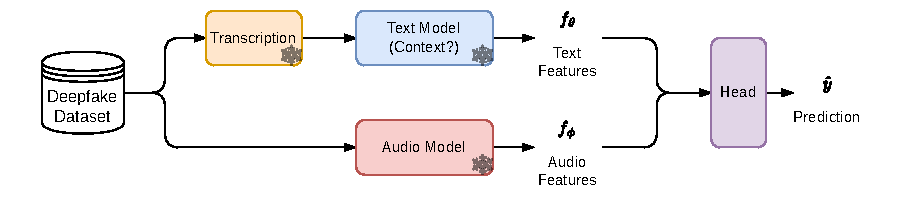
\includegraphics[width=0.8\textwidth]{figures/mid_fusion.pdf}
  \caption{Pipeline for Mid-Fusion. Features from the text and audio modules are concatenated and passed through an MLP to produce the final classification.}\label{fig:mid_fusion}
\end{figure*}

\begin{figure*}[t]
  \centering
  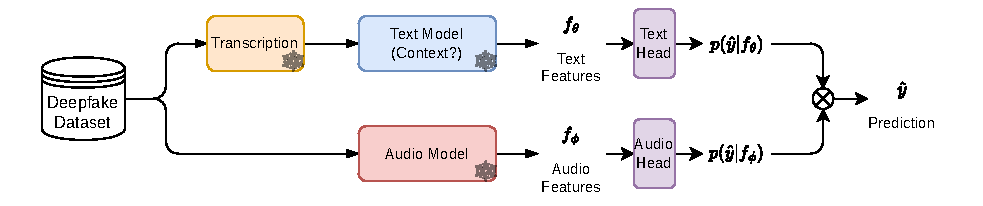
\includegraphics[width=0.8\textwidth]{figures/late_fusion.pdf}
  \caption{Pipeline for Late-Fusion. Predictions from the audio and text models are combined using a weighted mean to produce the final classification.}\label{fig:late_fusion} \todo[inline]{Abhay: I need to fix these arrowheads. Are centered captions better?}
\end{figure*}

\section{Experiments and Results}\label{sec:experiments_results}

\todo[inline]{Abhay: Need to decide whether we group by task\{text, audio, fusion\} or by \{datasets,metrics,baselines\}. Further, should we call the text model the `context module'?}

\subsection{Text / Context Module}
\subsubsection{Dataset}
For the authorship attribution task we incorporate an additional dataset
Wikiquotes, which provides a rich corpus of speeches from various authors.
Since only real samples are needed for training the text model, relying only on
the transcriptions provided by Whisper proved insufficient for learning the
nuanced characteristics of individual authors. \\
\subsubsection{Metrics}
ABX accuracy is a commonly used metric in speech and speaker representation
learning, often used in tasks related to contrastive learning. Similar to the
triplet loss we have three samples A,B and X. Where A and B are two embeddings
from different categories and X is a third representation, and the task is to
determine whether X is more similar to A or B based on the learned embeddings.
The accuracy measures the percentage of times the model correctly assigns X to
its corresponding label (closer to A or B). The decision rule is: $d(X,A) <
  d(X,B)$, where $d(x,y)$ is the distance function. \\
\subsubsection{Benchmark} We consider several state-of-the-art encoder-only architectures to benchmark
the effectiveness of the text model, including BERT, RoBERTa, DeBERTa, Modern
BERT, and the encoder of T5. Encoder-only models are particularly well-suited
for the task of authorship attribution because they focus exclusively on
encoding the input sequence into a fixed-size representation without
introducing additional complexities of the sequence-to-sequence
transformations. This focus allows them to better capture nuanced relationships
in the text, such as stylistic patterns and semantic coherence. We wanted to
identify the best architecture by comparing these models for capturing each
author's writing style and improving our detection system's overall
performance.

\todo[inline]{TODO @abhaydmathur : make gpu details fit.}
All experiments were conducted on a single NVIDIA A100 GPU with 40GB vRAM.

\section{Conclusions / Discussion}\label{sec:conclusions}

\newpage
\ifinterspeechfinal
  \section{Acknowledgements}
  Acknowledgement should only be included in the camera-ready version, not in the
  version submitted for review. The 5th page is reserved exclusively for
  acknowledgements and references. No other content must appear on the 5th page.
  Appendices, if any, must be within the first 4 pages. The acknowledgments and
  references may start on an earlier page, if there is space.

  \ifinterspeechfinal
    The Interspeech 2025 organisers
  \else
    The authors
  \fi
  would like to thank ISCA and the organising committees of past Interspeech conferences for their help and for kindly providing the previous version of this template.
\fi

\bibliographystyle{IEEEtran}
\bibliography{references}

\end{document}